\section{Global row minimality}\label{sec:upper-tail-row-minimality}

We use rooted densities to express the first-order density changes derived
by vertex insertion. Combining insertions with perturbations of the old
graphon, we obtain Lagrange multipliers and show that almost every row
of an upper-tail optimizer globally minimizes $\mathcal F_W$.

\subsection{Rooted densities and their gradients}\label{sec:rooted-densities}

\begin{figure}[htbp]
\centering
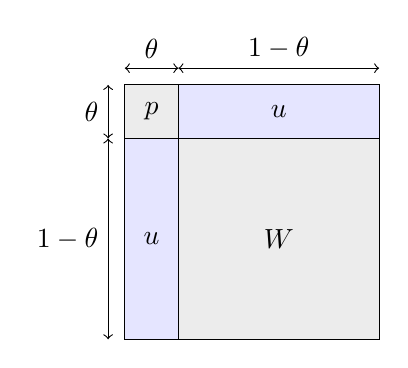
\begin{tikzpicture}[x=0.85cm,y=-0.85cm]
  \fill[gray!15] (0,0) rectangle (0.8,0.8);
  \fill[blue!10] (0.8,0) rectangle (3.8,0.8);
  \fill[blue!10] (0,0.8) rectangle (0.8,3.8);
  \fill[gray!15] (0.8,0.8) rectangle (3.8,3.8);
  \draw (0,0) rectangle (3.8,3.8);
  \draw (0.8,0) -- (0.8,3.8);
  \draw (0,0.8) -- (3.8,0.8);
  \node at (0.4,0.4) {$p$};
  \node at (2.3,0.4) {$u$};
  \node at (0.4,2.3) {$u$};
  \node at (2.3,2.3) {$W$};
  \draw[<->] (0,-0.25) -- node[above] {$\theta$} (0.8,-0.25);
  \draw[<->] (0.8,-0.25) -- node[above] {$1-\theta$} (3.8,-0.25);
  \draw[<->] (-0.25,0) -- node[left] {$\theta$} (-0.25,0.8);
  \draw[<->] (-0.25,0.8) -- node[left] {$1-\theta$} (-0.25,3.8);
\end{tikzpicture}
\caption{A new vertex class of mass $\theta$ has row $u$.
The old coordinates are rescaled to $[\theta,1]$.
The new block's internal value $p$ contributes
only at order $\theta^2$.}
\label{fig:insertion}
\end{figure}

Let $W$ be a graphon and let $u:[0,1]\to[0,1]$ be measurable.
The value $u(y)$ is the connection probability from a new vertex to an
old vertex with label $y \in [0,1]$.  To insert a new population of mass
$0\le\theta<1$, rescale the old labels to $[\theta,1]$ and define
\begin{equation}\label{eq:vertex-insertion}
  W_\theta(x,y):=
  \begin{cases}
    p, & 0\le x,y<\theta,\\
    u\!\left(\dfrac{x-\theta}{1-\theta}\right),
      & 0\le y<\theta\le x\le1,\\
    u\!\left(\dfrac{y-\theta}{1-\theta}\right),
      & 0\le x<\theta\le y\le1,\\
    W\!\left(\dfrac{x-\theta}{1-\theta},
               \dfrac{y-\theta}{1-\theta}\right),
      & \theta\le x,y\le1.
  \end{cases}
\end{equation}
\Cref{fig:insertion} illustrates this construction.

Copies of $H$ using no new vertex contribute $(1-\theta)^N t(H,W)$.
Those using at least two new vertices contribute $O(\theta^2)$, so
only copies using exactly one new vertex remain to be computed to
first order. If this vertex plays the role of $v\in V(H)$, its incident
edges use $u$ and all other edges use $W$. After rescaling the old
labels, these edge factors give the \emph{rooted density}
\begin{equation}\label{eq:rooted-density}
  \mathcal R_{H,W}^{v}(u):=\int_{[0,1]^{V(H)\setminus\{v\}}}
  \prod_{z\in N_H(v)}u(x_z)
  \prod_{\substack{ab\in E(H)\\ a,b\ne v}}W(x_a,x_b)
  \prod_{z\in V(H)\setminus\{v\}}\dd x_z,
\end{equation}
with root $v$ and row $u$. The corresponding mass factor is
$\theta(1-\theta)^{N-1}$. Summing over all possible roots gives
\begin{equation}\label{eq:total-rooted-density}
  \mathcal R_{H,W}(u):=\sum_{v\in V(H)}\mathcal R_{H,W}^{v}(u),
\end{equation}
which we also call the \emph{rooted density} when the root is unspecified.

Combining the contributions from zero and one new vertex gives
\begin{equation}\label{eq:insertion-density-expansion}
  t(H,W_\theta)=(1-\theta)^N t(H,W)
  +\theta(1-\theta)^{N-1}\mathcal R_{H,W}(u)+O(\theta^2).
\end{equation}
Differentiating at $\theta=0$ gives
\begin{equation}\label{eq:insertion-density-derivative}
  \left.\frac{\dd}{\dd\theta}t(H,W_\theta)\right|_{\theta=0^+}
  =\mathcal R_{H,W}(u)-Nt(H,W).
\end{equation}
Thus $\mathcal R_{H,W}(u)$ is the contribution of the inserted row to the
first-order density change, while $-Nt(H,W)$ accounts for reducing the
mass of the old vertices from $1$ to $1-\theta$.

The integral in~\eqref{eq:rooted-density} also defines the rooted
density for $W\in L^\infty_{\mathrm{sym}}([0,1]^2)$ and
$u\in L^\infty([0,1])$. For fixed $W$, its $d_v$ factors of $u$
make $\mathcal R_{H,W}^{v}$ a continuous polynomial functional of $u$,
homogeneous of degree $d_v$.
Summing over roots gives a polynomial functional
$\mathcal R_{H,W}$ of degree at most $\Delta(H)$.

At $u=W_x$, the value $\mathcal R_{H,W}^{v}(W_x)$ is the usual
homomorphism density rooted at $v$ with label $x$, as introduced
in~\cite{LovaszGraphLimits}.  Integrating over $x$ gives $t(H,W)$
for each root, so
\begin{equation}\label{eq:rooted-average}
  \int_0^1\mathcal R_{H,W}(W_x)\dd x=N\,t(H,W).
\end{equation}

To measure how the rooted density $\mathcal R_{H,W}(u)$ changes with respect to the row $u$,
keep $W$ fixed and perturb $u$ to $u+\zeta h$, where $h\in L^\infty([0,1])$.
Then the integral in~\eqref{eq:rooted-density} is polynomial in $\zeta$;
its derivative at zero defines
\[
  D\mathcal R_{H,W}^{v}(u)[h]:=
  \left.\frac{\dd}{\dd\zeta}
    \mathcal R_{H,W}^{v}(u+\zeta h)\right|_{\zeta=0}.
\]
Only the factors corresponding to edges incident to $v$ depend on
$\zeta$.  The product rule gives
\[
  \left.\frac{\dd}{\dd\zeta}
    \prod_{z\in N_H(v)}\bigl(u(x_z)+\zeta h(x_z)\bigr)
  \right|_{\zeta=0}
  =\sum_{z_0\in N_H(v)}h(x_{z_0})
    \prod_{z\in N_H(v)\setminus\{z_0\}}u(x_z).
\]
Substituting into~\eqref{eq:rooted-density} and applying Fubini's theorem gives
\begin{align*}
  D\mathcal R_{H,W}^{v}(u)[h]
  &=\sum_{z_0\in N_H(v)}
    \int_{[0,1]^{V(H)\setminus\{v\}}}
    h(x_{z_0})\prod_{z\in N_H(v)\setminus\{z_0\}}u(x_z)
    \prod_{\substack{ab\in E(H)\\ a,b\ne v}}W(x_a,x_b)
    \prod_{z\in V(H)\setminus\{v\}}\dd x_z\\
  &=\sum_{z_0\in N_H(v)}\int_0^1G_{v,z_0}(u)(y)h(y)\dd y,
\end{align*}
where we isolate the kernel $G_{v,z_0}(u)$ associated with the oriented edge $vz_0$: for $y\in[0,1]$,
\begin{equation}\label{eq:rooted-gradient-kernel}
  G_{v,z_0}(u)(y):=\int_{[0,1]^{V(H)\setminus\{v,z_0\}}}\prod_{z\in N_H(v)\setminus\{z_0\}}u(x_z)
  \prod_{\substack{ab\in E(H)\\ a,b\ne v}}W(x_a,x_b)
  \prod_{z\in V(H)\setminus\{v,z_0\}}\dd x_z,
  \qquad x_{z_0}=y.
\end{equation}
Summing over $v\in V(H)$ defines the gradient $\nabla\mathcal R_{H,W}(u)$
and the directional derivative $D\mathcal R_{H,W}(u)[h]$:
\begin{align*}
  \nabla\mathcal R_{H,W}(u) &:=\sum_{v\in V(H)}\sum_{z_0\in N_H(v)}G_{v,z_0}(u), \\
  D\mathcal R_{H,W}(u)[h] &:=\sum_{v\in V(H)}D\mathcal R_{H,W}^{v}(u)[h]
  =\int_0^1\nabla\mathcal R_{H,W}(u)(y)h(y)\dd y.
\end{align*}
The number of terms in $\nabla\mathcal R_{H,W}(u)$ is $\sum_v d_v=2m$,
and each term $G_{v,z_0}(u)$ lies in $[0,1]$ when $W\in\W_0$
and $0\le u\le1$. Hence
\begin{equation}\label{eq:rooted-gradient-bound}
  0\le\nabla\mathcal R_{H,W}(u)\le2m.
\end{equation}
Integrating the derivative along a segment gives
\[
  \mathcal R_{H,W}(u)-\mathcal R_{H,W}(u')
  =\int_0^1\int_0^1
    \nabla\mathcal R_{H,W}\bigl(u'+\theta(u-u')\bigr)(y)
    (u(y)-u'(y))\dd y\dd\theta.
\]
Consequently, for $[0,1]$-valued measurable $u,u'$,
\begin{equation}\label{eq:rooted-lipschitz}
  |\mathcal R_{H,W}(u)-\mathcal R_{H,W}(u')|\le2m\|u-u'\|_1,
\end{equation}
so $\mathcal R_{H,W}$ is $2m$-Lipschitz with respect to the $L^1([0,1])$ norm.

The gradient also satisfies a Lipschitz bound from $L^1([0,1])$ to $L^\infty([0,1])$.
For $[0,1]$-valued measurable $u,u'$, apply~\eqref{eq:product-difference}
to the $k=d_v-1$ factors of $u$ and $u'$ in~\eqref{eq:rooted-gradient-kernel}.
Since all other factors lie in $[0,1]$, integrating each summand gives
a function with $L^\infty([0,1])$-norm at most $\|u-u'\|_1$.  Thus
\[
  \|G_{v,z_0}(u)-G_{v,z_0}(u')\|_\infty
  \le(d_v-1)\|u-u'\|_1.
\]
Summing over $v$ and $z_0\in N_H(v)$, and using
$\sum_v d_v(d_v-1)\le2m(\Delta(H)-1)$, gives
\begin{equation}\label{eq:gradient-lipschitz}
  \|\nabla\mathcal R_{H,W}(u)-\nabla\mathcal R_{H,W}(u')\|_\infty
  \le2m(\Delta(H)-1)\|u-u'\|_1.
\end{equation}

\begin{expl}\label{expl:triangle-rooted}
For $H=K_3$ and $u : [0,1]\to[0,1]$ measurable, the rooted density and its gradient are
\[
  \mathcal R_{H,W}(u)=3\int_{[0,1]^2}W(y,z)u(y)u(z)\dd y\dd z,
  \qquad
  \nabla\mathcal R_{H,W}(u)(y)=6\int_0^1W(y,z)u(z)\dd z.
\]
Since $m=3$ for $K_3$, we obtain $0\le\nabla\mathcal R_{H,W}(u)\le6$
as in \eqref{eq:rooted-gradient-bound}.
\end{expl}

\begin{expl}\label{expl:path-rooted}
Let $H=P_3$ be the three-vertex path.
For measurable $u:[0,1]\to[0,1]$, rooting at the middle vertex or at
an endpoint gives, respectively,
\[
  \mathcal R_{H,W}^{\text{mid}}(u)=\left(\int_0^1u(y)\dd y\right)^2,
  \qquad
  \mathcal R_{H,W}^{\text{end}}(u)=\int_0^1d_W(y)u(y)\dd y.
\]
Consequently, the rooted density and its gradient are
\[
  \mathcal R_{H,W}(u)
  =\left(\int_0^1u(y)\dd y\right)^2
    +2\int_0^1d_W(y)u(y)\dd y,
  \qquad
  \nabla\mathcal R_{H,W}(u)(y)
  =2\Bigl(\int_0^1u(z)\dd z+d_W(y)\Bigr).
\]
Since $m=2$ for $P_3$, we obtain $0\le\nabla\mathcal R_{H,W}(u)\le4$
as in \eqref{eq:rooted-gradient-bound}.
\end{expl}

\subsection{Lagrange multipliers}\label{sec:lagrange-multipliers}

For the rest of this section, fix an upper-tail minimizer $W$ as in
\Cref{sec:upper-tail-interiority}.
Retain the notation $t_j$ and $\mathcal A$ for the constrained densities of $H_j$
and active indices, and write $N_j:=|V(H_j)|$.
For measurable $u:[0,1]\to[0,1]$, define
\begin{equation}\label{eq:insertion-rates}
  a_j(u):=\mathcal R_{H_j,W}(u)-N_jt_j(W),\qquad b(u):=2\bigl(I_p(u)-I_p(W)\bigr).
\end{equation}
By~\eqref{eq:insertion-density-derivative}, $a_j(u)$ is the derivative
at $\theta=0^+$ of the $H_j$-density under insertion of the single row $u$.
The coefficient $b(u)$ gives the corresponding derivative of the entropy cost.
Each quantity in \eqref{eq:insertion-rates}
subtracts the contribution lost by reducing the mass of the old
vertices from the contribution of the new row.  Thus $a_j(u)>0$ indicates
a density increase, while $b(u)<0$ indicates a cost decrease, to first order.
When the old graphon is also replaced by $W+\theta V$, its first-order
contributions are $Dt_j(W)[V]$ and $DI_p(W)[V]$.

\begin{lemma}\label{lem:insertion-first-order}
Let $W$ be a minimizer of~\eqref{eq:joint-variational-problem}, let $u_1,\dots,u_k$ be
measurable functions from $[0,1]$ to $[0,1]$, let $c_1,\dots,c_k\ge0$, and let
$V\in L^\infty_{\mathrm{sym}}([0,1]^2)$.  There are $\theta_0>0$ and graphons $W_\theta$
for $0\le\theta<\theta_0$, with $W_0=W$, such that for every $1\le j\le s$,
\begin{align*}
  t_j(W_\theta)&=t_j(W)
  +\theta\Bigl(\sum_{i=1}^kc_ia_j(u_i)+Dt_j(W)[V]\Bigr)+O(\theta^2), \\
  I_p(W_\theta)&=I_p(W)
  +\theta\Bigl(\sum_{i=1}^kc_ib(u_i)+DI_p(W)[V]\Bigr)+O(\theta^2).
\end{align*}
\end{lemma}

\begin{proof}
Put $c:=\sum_ic_i$.  For $\theta>0$ with $\theta c<1$, partition
$[0,\theta c)$ into consecutive intervals $I_1,\dots,I_k$ of lengths $\theta c_i$ and
rescale the old graphon to $[\theta c,1]$, as in
\eqref{eq:vertex-insertion}.  Replace its values by $W+\theta V$.
Define
\[
  W_\theta(x,y):=
  \begin{cases}
    p, & 0\le x,y<\theta c,\\
    u_i\!\left(\dfrac{x-\theta c}{1-\theta c}\right),
      & y\in I_i,\ \theta c\le x\le1,\\
    u_i\!\left(\dfrac{y-\theta c}{1-\theta c}\right),
      & x\in I_i,\ \theta c\le y\le1,\\
    (W+\theta V)\!\left(\dfrac{x-\theta c}{1-\theta c},
                          \dfrac{y-\theta c}{1-\theta c}\right),
      & \theta c\le x,y\le1.
  \end{cases}
\]
By \Cref{lem:upper-tail-basic}, $p\le W\le1-\gamma$, so for small
$\theta>0$ this defines a graphon $W_\theta$.

Grouping copies of $H_j$ by their new vertices, as in
\eqref{eq:insertion-density-expansion}, gives
\[
  t_j(W_\theta) =(1-\theta c)^{N_j}t_j(W+\theta V)+\theta(1-\theta c)^{N_j-1}
  \sum_ic_i\mathcal R_{H_j,W}(u_i)+O(\theta^2).
\]
The two explicit terms come from copies with no new vertex and with
exactly one new vertex.  In the latter, replacing the old edge factors
$W+\theta V$ by $W$ changes each integral by $O(\theta)$, which is
multiplied by the new interval's mass $\theta c_i$.
Copies with at least two new vertices also contribute $O(\theta^2)$.
Using
\[
  (1-\theta c)^{N_j}=1-\theta cN_j+O(\theta^2),\qquad
  t_j(W+\theta V)=t_j(W)+\theta Dt_j(W)[V]+O(\theta^2)
\]
and $c=\sum_i c_i$, we obtain
\begin{align*}
    t_j(W_\theta)
    &=t_j(W)+\theta\sum_i c_i\mathcal R_{H_j,W}(u_i)-\theta cN_jt_j(W)
      +\theta Dt_j(W)[V]+O(\theta^2)\\
    &=t_j(W)+\theta \left( \sum_i c_i a_j(u_i) + Dt_j(W)[V] \right) +O(\theta^2).
\end{align*}
The entropy has the exact expression
\[
  I_p(W_\theta)=(1-\theta c)^2I_p(W+\theta V)
  +2\theta(1-\theta c)\sum_ic_i I_p(u_i).
\]
Since $J_p(p)=0$, pairs of new vertices contribute zero.
Using
\[
  (1-\theta c)^2=1-2\theta c+O(\theta^2),\qquad
  I_p(W+\theta V)=I_p(W)+\theta DI_p(W)[V]+O(\theta^2),
\]
we obtain
\begin{align*}
    I_p(W_\theta)
    &=I_p(W)+2\theta\Bigl(\sum_i c_i I_p(u_i)-cI_p(W)\Bigr)
      +\theta DI_p(W)[V]+O(\theta^2)\\
    &=I_p(W)+\theta \left( \sum_i c_i b(u_i) + DI_p(W)[V] \right) +O(\theta^2).
\end{align*}
In each expansion, the three first-order terms come, respectively,
from adding the new rows, reducing the mass of the old vertices from
$1$ to $1-\theta c$, and perturbing the old graphon by $\theta V$.
\end{proof}

No combination of row insertions and perturbations of the old graphon
can decrease the entropy cost and strictly increase every active density
to first order: for small $\theta>0$, it would give a feasible
competitor with lower cost. Separating these forbidden changes from
those in \Cref{lem:insertion-first-order} gives the following multipliers.

\begin{lemma}[Lagrange multipliers]\label{lem:upper-tail-multiplier}
Let $W$ be a minimizer of~\eqref{eq:joint-variational-problem}.
There are $\mu_1,\dots,\mu_s\ge0$, with $\mu_j=0$ for inactive $j$, such that
\begin{enumerate}[label=(\roman*)]
  \item $J_p'(W(x,y))=\sum_{j=1}^s\mu_j\mathcal D_{H_j,W}(x,y) \quad\text{for almost every }(x,y)\in[0,1]^2$,
  \item $b(u)-\sum_{j=1}^s\mu_ja_j(u)\ge0 \quad\text{for every measurable }u:[0,1]\to[0,1]$,
  \item if $W\not\equiv p$, then $\sum_{j=1}^s\mu_j>0$.
\end{enumerate}
\end{lemma}

\begin{proof}
Let $\mathcal C\subseteq\RR^{1+s}$ be the set of vectors $z=(z_0,\dots,z_s)$
whose coordinates have the form
\[
  z_0=\sum_{i=1}^k c_i b(u_i)+DI_p(W)[V],
  \qquad z_j=\sum_{i=1}^k c_i a_j(u_i)+Dt_j(W)[V], \qquad 1\le j\le s,
\]
over all finite families of measurable $u_i:[0,1]\to[0,1]$, coefficients
$c_i\ge0$, and $V\in L^\infty_{\mathrm{sym}}([0,1]^2)$.  Then $\mathcal C$ is a convex cone: adding two such
vectors amounts to concatenating the families and adding the perturbations.
It also contains $0$ and all changes arising from either $V$ or $-V$ with no insertion.

The directions that strictly improve the cost and all active constraints form
\[
  \mathcal N:=\bigl\{z\in\RR^{1+s}:z_0<0\text{ and }z_j>0\text{ for every }j\in\mathcal A\bigr\},
\]
an open convex cone disjoint from $\mathcal C$.  Suppose that
$z\in\mathcal C\cap\mathcal N$ is realized by a family $(u_i,c_i)$ and a
perturbation $V$, and let $W_\theta$ be as in
\Cref{lem:insertion-first-order}.  For each active $j$,
\[
  t_j(W_\theta)=r_j^{m_j}+\theta z_j+O(\theta^2)>r_j^{m_j}
\]
when $\theta>0$ is small.  The inactive constraints remain satisfied by
continuity, so $W_\theta$ is feasible.  On the other hand, when $\theta>0$ is small,
\[
  I_p(W_\theta)=I_p(W)+\theta z_0+O(\theta^2)<I_p(W),
\]
contradicting minimality.

Since $\mathcal C$ is convex, $\mathcal N$ is open and
convex, and the two are disjoint, a hyperplane separates them.
Both cones have $0$ in their closures, so this hyperplane passes through
the origin.  Write its equation as
\[
  \lambda z_0-\sum_j\mu_jz_j=0,\qquad
  (\lambda,\mu_1,\dots,\mu_s)\ne0.
\]
Choose the signs of the coefficients so that
\begin{equation}\label{eq:separated-cones}
  \lambda z_0-\sum_j\mu_jz_j\ge0\quad(z\in\mathcal C),\qquad
  \lambda z_0-\sum_j\mu_jz_j\le0\quad(z\in\mathcal N).
\end{equation}
By continuity, the latter inequality also holds on $\overline{\mathcal N}$.
The following permitted values in $\overline {\mathcal N}$,
obtained by fixing a single coordinate while letting the other coordinates be zero, give
\[
  z_0=-1 \implies \lambda\ge0,
  \qquad z_j=1,\ j\in\mathcal A \implies \mu_j\ge0,
  \qquad z_j=\pm1,\ j\notin\mathcal A \implies \mu_j=0.
\]
Setting $c_i=0$ for all $i$ and using the perturbations $V$ and $-V$, we obtain two vectors
\[
  \pm\,(DI_p(W)[V],\ Dt_1(W)[V],\ \dots,\ Dt_s(W)[V])\in\mathcal C.
\]
Since both vectors belong to $\mathcal C$, the first inequality
in~\eqref{eq:separated-cones} must hold with equality for both.
They therefore lie on the separating hyperplane, giving
\begin{equation}\label{eq:separated-el}
  \lambda\,DI_p(W)[V]=\sum_{j=1}^s\mu_j\,Dt_j(W)[V]
  \qquad (V\in L^\infty_{\mathrm{sym}}([0,1]^2)).
\end{equation}
Taking $V=\mathbf 1$, since $W \ge p$ almost everywhere, we have
\[
  Dt_j(W)[\mathbf1]=\int\mathcal D_{H_j,W} \ge m_jp^{m_j-1}>0.
\]
If $\lambda=0$, \eqref{eq:separated-el} would imply
\[
  0=\sum_j\mu_j Dt_j(W)[\mathbf1]
    \ge\sum_j\mu_jm_jp^{m_j-1},
\]
forcing every $\mu_j$ to vanish, which is impossible since
$(\lambda,\mu_1,\dots,\mu_s)\ne0$.  We may therefore normalize
$\lambda=1$. By \Cref{lem:upper-tail-basic}, the symmetric kernel
$J_p'(W)-\sum_j\mu_j\mathcal D_{H_j,W}$ is bounded.
Substituting this kernel for $V$ in~\eqref{eq:separated-el} and writing
the derivatives as integrals gives
\[
  \int_{[0,1]^2}\left|J_p'(W)-\sum_j\mu_j\mathcal D_{H_j,W}\right|^2=0,
\]
which proves part~\textit{(i)}.

Taking $k=1$, $c_1=1$, $u_1=u$, and $V=0$ gives a vector $(b(u), a_1(u),\dots,a_s(u))\in\mathcal C$,
and substituting it into \eqref{eq:separated-cones} gives $b(u)-\sum_j\mu_ja_j(u)\ge0$,
proving part~\textit{(ii)}.
Finally, if every $\mu_j$ vanishes, part~\textit{(ii)} with $u\equiv p$ gives
\[
  0\le b(p)=-2I_p(W).
\]
Hence $W=p$ almost everywhere, proving part~\textit{(iii)}.
\end{proof}

\subsection{Global row minimality}\label{sec:row-minimality}

For the multipliers in \Cref{lem:upper-tail-multiplier} and measurable $u:[0,1]\to[0,1]$,
define $\mathcal F_W$ by
\begin{equation}\label{eq:row-functional}
  \mathcal F_W(u):=b(u)-\sum_{j=1}^s\mu_j a_j(u)
  =2\bigl(I_p(u)-I_p(W)\bigr)-\sum_{j=1}^s\mu_j\bigl(\mathcal R_{H_j,W}(u)-N_jt_j(W)\bigr).
\end{equation}
In the construction of \Cref{lem:insertion-first-order},
insert one row $u$ with mass $\theta$ and replace the old graphon by
$W+\theta V$. Part~\textit{(i)} of \Cref{lem:upper-tail-multiplier} gives
\[
  DI_p(W)[V]-\sum_{j=1}^s\mu_jDt_j(W)[V]=0.
\]
Thus the first-order entropy change minus the weighted density changes
depends only on the inserted row and equals $\mathcal F_W(u)$: the
contributions from perturbing the old graphon cancel.

\begin{lemma}[Global row minimality]\label{lem:global-row-minimality}
For $W$ and the multipliers constructed in
\Cref{lem:upper-tail-multiplier}, one has
\begin{equation*}
  \mathcal F_W(u)\ge0
  \qquad\text{for every measurable }u:[0,1]\to[0,1],
\end{equation*}
with equality for almost every row $u=W_x$.
\end{lemma}

\begin{proof}
Part~\textit{(ii)} of \Cref{lem:upper-tail-multiplier} gives
$\mathcal F_W(u)\ge0$ for every measurable $u:[0,1]\to[0,1]$.
By~\eqref{eq:insertion-rates}, Fubini's theorem and~\eqref{eq:rooted-average},
\[
  \int_0^1a_j(W_x)\dd x=0,\qquad \int_0^1b(W_x)\dd x=0.
\]
Hence $\int_0^1\mathcal F_W(W_x)\dd x=0$.  Since the integrand is
nonnegative, it vanishes almost everywhere, proving the equality assertion.
\end{proof}
